\documentclass{beamer}
\usepackage{beamerthemeshadow}
\usepackage[utf8]{inputenc}
\usepackage[T1]{fontenc}
\usepackage{tikz}
\usepackage{cmbright}
\usepackage{mhchem}
\usepackage{braket}
\usepackage{biblatex}
\addbibresource{slide_cite.bib}
\fontencoding{OT1}\fontfamily{cmbr}\selectfont %to load ot1cmbr.fd
\DeclareFontShape{OT1}{cmbr}{bx}{n}{% change bx definition
<->cmbrbx10%
}{}
\normalfont % back to normalfont

\setbeamertemplate{navigation symbols}{}
\setbeamertemplate{section in toc}[sections numbered]
\setbeamertemplate{subsection in toc}[subsections numbered]
\setbeamertemplate{footline}[frame number]

\newcommand\Fontvi{\fontsize{8}{7.2}\selectfont} %font size changer

%font type:
\newenvironment{ppl}{\fontfamily{ppl}\selectfont}{\par}


% macros:
\def\D{\displaystyle}
\def\att{                    % mark at the margin
        \marginpar[ \hspace*{\fill} \raisebox{-0.2em}{\rule{2mm}{1.2em}} ]
        {\raisebox{-0.2em}{\rule{2mm}{1.2em}} }
        }
\def\at#1{[*** \att #1 ***]}  % text needing attention
\def\spc{\hspace*{0.5cm}} 			% indentation


%Information to be included in the title page:
\title{Potential energy surface of H$_x$O$_y$}
\author[Aribowo, Neumaier] % (optional, for multiple authors)
{Beryl Ramadhian Aribowo}

\institute[VFM] % (optional)
{
    Supervised by Prof. Arnold Neumaier\\
    Faculty of Mathematics\\
    University of Vienna
}
%\date[VGSCO 2021] % (optional)
%{VGSCO Seminar}

\date{17 December 2021}


\begin{document}

\frame{\titlepage}

\begin{frame}
    \frametitle{Outline}
    \begin{columns}[t]
        \begin{column}{.5\textwidth}
            \tableofcontents[sections={1-2}]
        \end{column}
        \begin{column}{.5\textwidth}
            \tableofcontents[sections={3-5}]
        \end{column}
    \end{columns}
\end{frame}


\section{Introduction}
\subsection{Atoms \& molecules}
\iffalse
\begin{frame}{Nuclear geometry}
    \begin{itemize}
        \item Nuclear geometry
    \end{itemize}
    \begin{figure}[htbp]
        \centering
        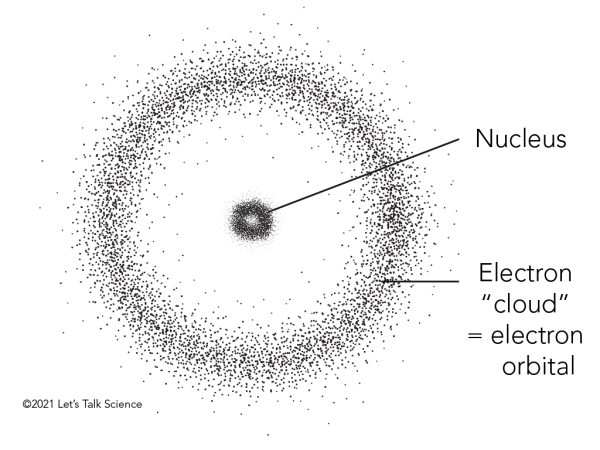
\includegraphics[scale=0.5]{img/slide/electron_cloud.png}
        \label{fig:nucleargeometry}
    \end{figure}
\end{frame}
\fi

\begin{frame}{H$_x$O$_y$}
    \begin{columns}
        \begin{column}{0.5\textwidth}
            \begin{itemize}
                \item Goal: To construct general, cheap, and accurate mathematical models for global potential energy surfaces of H$_x$O$_y$ molecules.
                \item Examples of H$_x$O$_y$: H$_2$, O$_2$, O$_3$, OH, H$_2$O, H$_2$O$^+$, HO$_2^+$, H$_2$O$_2$, etc.
            \end{itemize}
        \end{column}
        \begin{column}{0.5\textwidth}
            \begin{figure}[htbp]
                \centering
                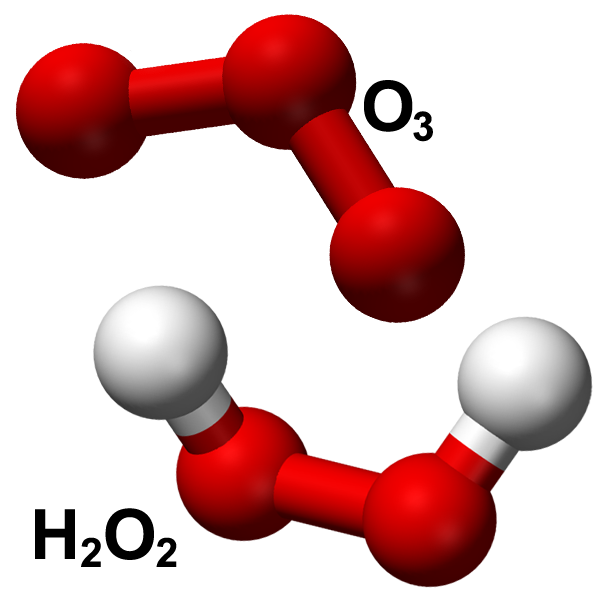
\includegraphics[scale=0.3]{img/slide/ozone.png}
                \label{fig:ozone}
            \end{figure}
        \end{column}
    \end{columns}
\end{frame}

\begin{frame}{Atom type}
    \begin{itemize}
        \item Atom type
        \begin{figure}[htbp]
            \centering
            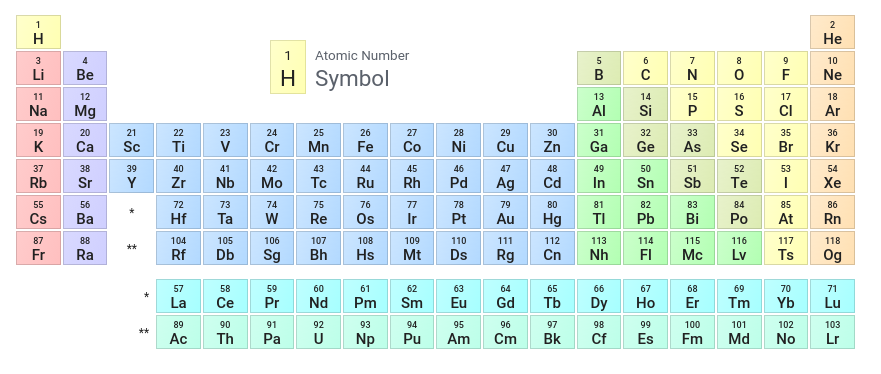
\includegraphics[scale=0.3]{img/slide/periodic_table.png}
            \label{fig:h2o}
        \end{figure}
        \item $Z_\text{atom} = $ atomic number.
    \end{itemize}
\end{frame}

\begin{frame}{Important quantities}
    \begin{itemize}
        \item Molecular structure
        \begin{figure}[htbp]
            \centering
            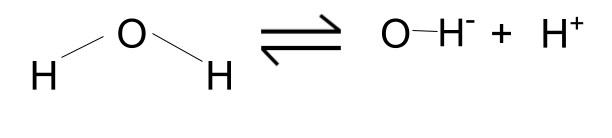
\includegraphics[scale=0.3]{img/slide/molecular_structure.png}
            \label{fig:h2o}
        \end{figure}
        \item Interatomic distance:
        \begin{equation}
            r_{ij} = ||\mathbf{x}_i - \mathbf{x}_j||_2,
        \end{equation}
        where
        \begin{equation}
            ||\mathbf{x}||_2 = \sqrt{x_1^2 + x_2^2 + x_3^2}.
        \end{equation}
        \item $\mathbf{R} = (R_{12}, R_{13},...R_{n-1,n})$.
        %\item $R_k \in R_{ij}$ $(k = 1,2,3...)$ refers to data points.
    \end{itemize}
\end{frame}

\subsection{Potential energy surface (PES)}
\begin{frame}{PES}
    \Fontvi
    \textbf{Potential energy surface (PES)}, in the simplest form:
    \begin{equation}
        V := V(\mathbf{R}),
    \end{equation}
    \begin{itemize}
        \item Properties:
        \begin{itemize}
            \Fontvi
            \item Single valued
            \item Smooth (except at conical intersections)
            \item Finite except when two nuclei positions are equal.
            \item \textbf{Permutation symmetric}
        \end{itemize}
        \item Categories:
        \begin{itemize}
            \Fontvi
            \item Local PES: short range only or within the bond length (molecular vibration, rotation, translation, and most reactions).
            \item Global PES: no range restrictions.
        \end{itemize}
        \item \textbf{Force} on atom $i$ = partial derivative of potential energy with respect to the coordinate of the atom $i$.
        \item \textbf{Force field} = gradient of PES.
    \end{itemize}
    
\end{frame}
\begin{frame}{PES}
    \begin{figure}[htbp]
        \centering
        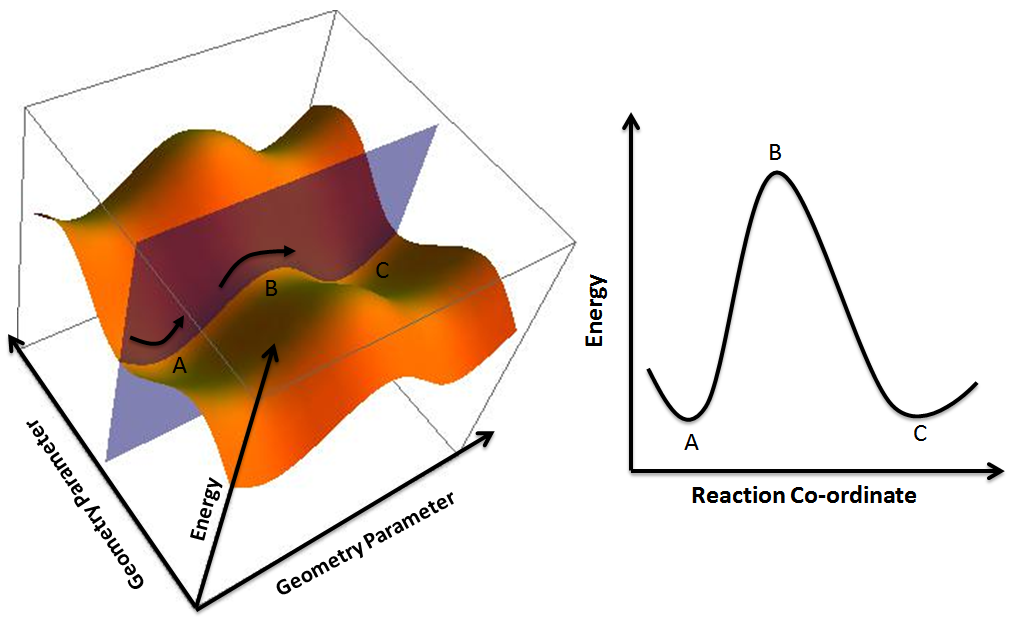
\includegraphics[scale=0.2]{img/slide/pes.png}
        \label{fig:pes}
    \end{figure}
    Observables:
    \begin{itemize}
        \item Minimum point, \textbf{force} = 0:
        \begin{itemize}
            \item local = metastable
            \item global = stable
        \end{itemize}
        \item Saddle point = transition state:
            \begin{itemize}
                \item Molecular vibration, translation, and rotation, if bounded.
                \item Bond-breaking/making, if unbounded.
            \end{itemize}
    \end{itemize}
\end{frame}
\begin{frame}{Applications of PES}
    \begin{figure}[htbp]
        \centering
        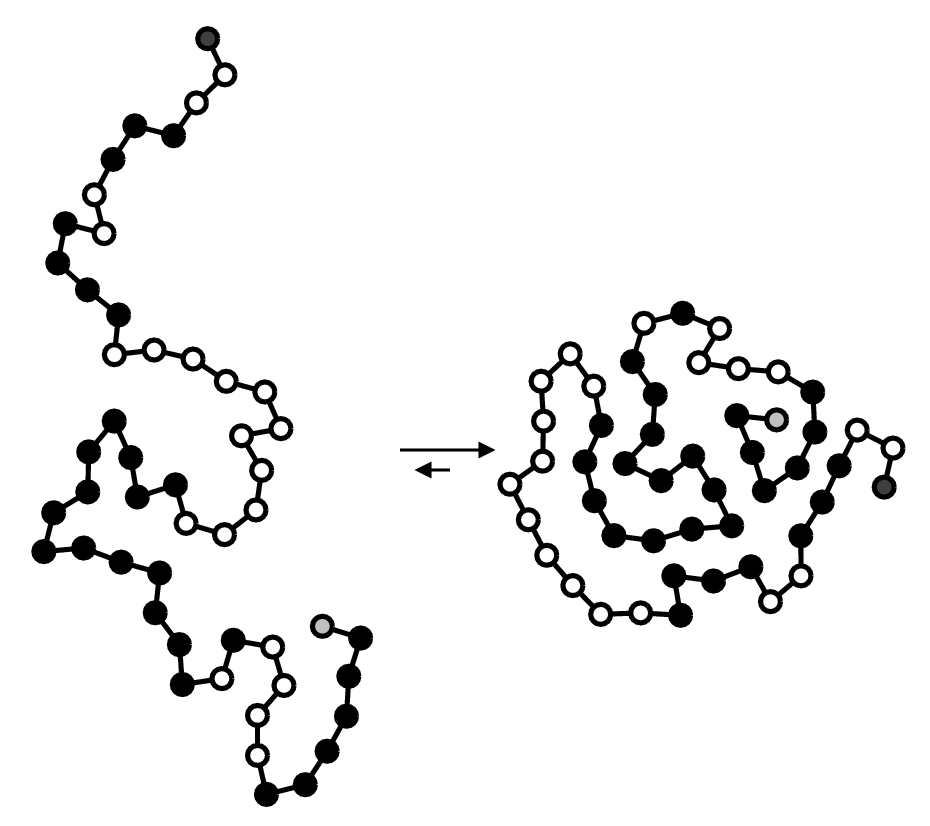
\includegraphics[scale=0.15]{img/slide/Protein_folding_schematic.png}
        \label{fig:pes}
    \end{figure}
    \begin{itemize}
        \item Molecular dynamics: protein folding, drug discovery, etc. Needs millions of function evaluations!
        \item Example: CHARMM force field.
    \end{itemize}
    Cheap and accurate functional form is important!
\end{frame}

\subsection{Examples of pair potential curves}
\begin{frame}{H$_2$ curves}
    \begin{figure}[h]
        \centering
        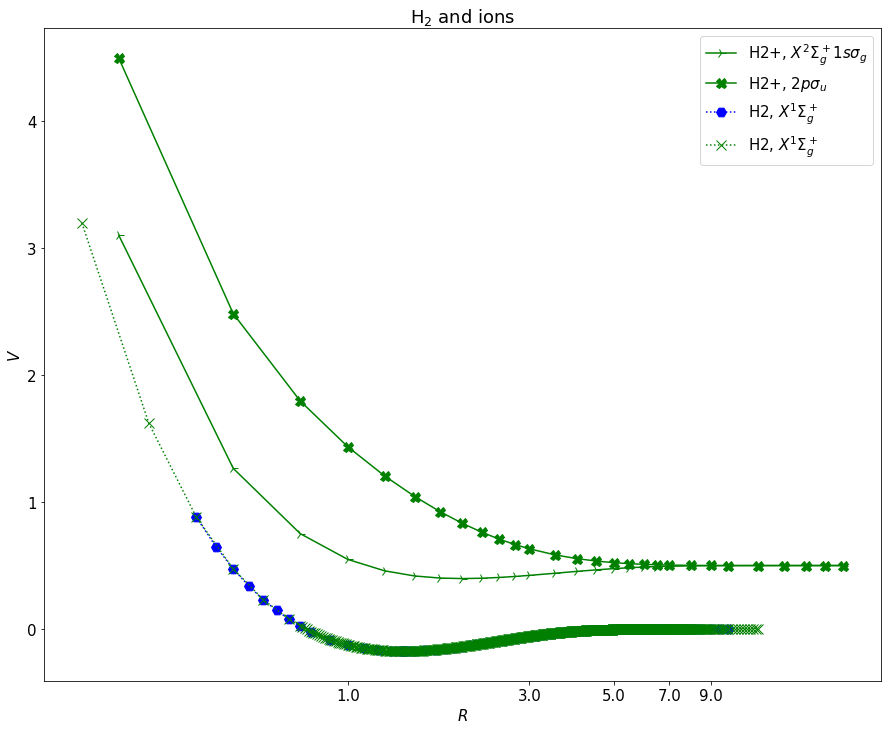
\includegraphics[scale=0.27]{img/H2_and_ions.png}
        \label{fig:h2}
    \end{figure}
\end{frame}
\begin{frame}{Spectroscopic notation \& energy level}
    \begin{itemize}
        \item The spectroscopic notation encodes quantum mechanics properties: the symmetry properties of wave function.
        \item Spectroscopic notation:
        \begin{itemize}
            \item States:
            \begin{itemize}
                \item Ground state: $X$
                \item Excited state: $A, B, C,$...
            \end{itemize}
            \item $2S+1$ spin multiplicity.
            \item Angular momentum $\Lambda$: $\Sigma, \Pi, \Delta, \Phi ... $ (follows $s, p, d, f...$) signify $\Lambda = 0, 1, 2, 3 ...$ respectively.
            \item Reflection: $+$ (symmetric), $-$ (anti-symmetric).
            \item Parity: $g$ (even), $u$ (odd).
            \item Examples: H$_2(X^1\Sigma_g^+)$, H$_2^+(X^2\Sigma_g^+)$, O$_2^+(X^2\Pi_g)$.
        \end{itemize}
    \end{itemize}
\end{frame}
\begin{frame}{O$_2$ curves}
    \begin{figure}[h]
        \centering
        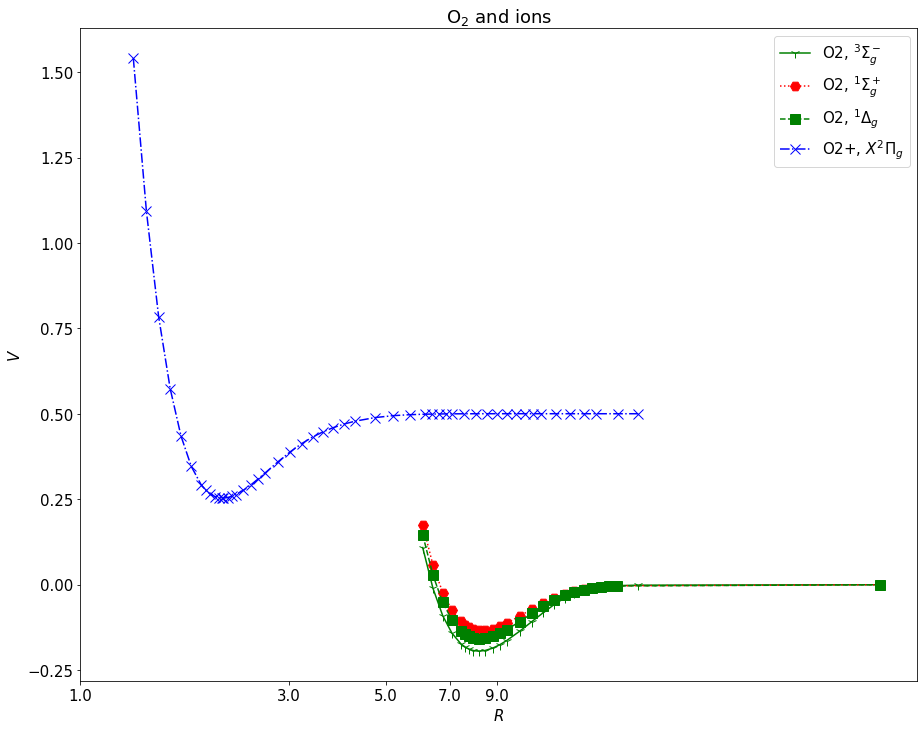
\includegraphics[scale=0.27]{img/O2_and_ions.png}
        \label{fig:o2}
    \end{figure}
\end{frame}
\begin{frame}{OH curves}
    \begin{figure}[h]
        \centering
        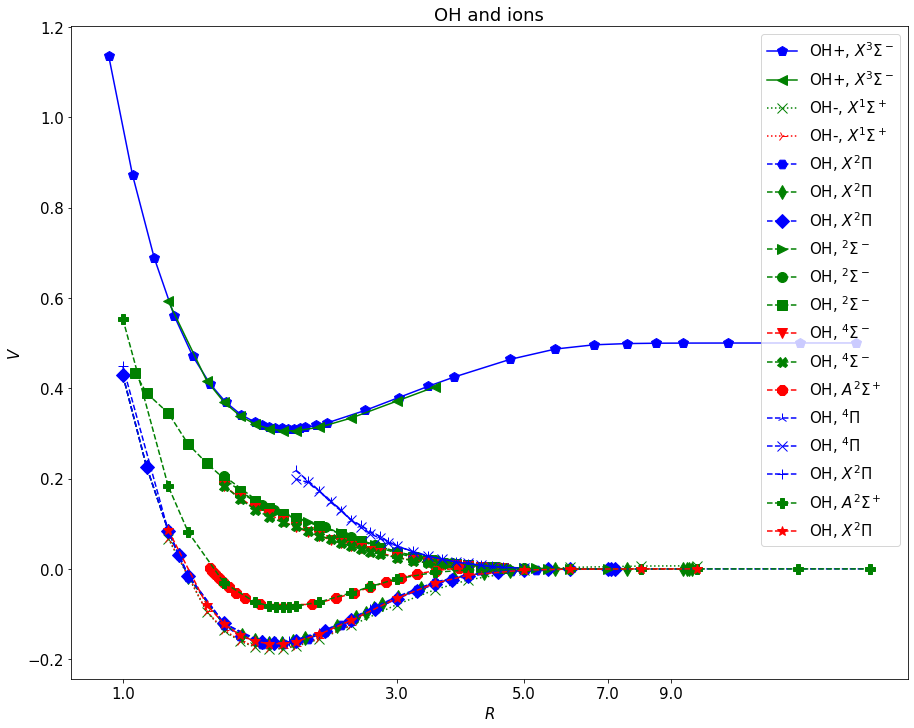
\includegraphics[scale=0.27]{img/OH_and_ions.png}
        \label{fig:oh}
    \end{figure}
\end{frame}

\iffalse
\begin{frame}{Breakdown of classical mechanics}
    \begin{figure}[htbp]
        \centering
        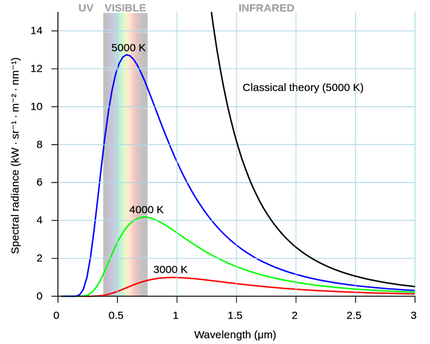
\includegraphics[scale=0.4]{img/slide/blackbody.png}
        \label{fig:pes}
    \end{figure}
    Breakdown of classical mechanics (black body radiation) $\rightarrow$ energy discretization (quantization of energy) $\rightarrow$ the Schrödinger eq $\rightarrow$ Born interpretation. 
\end{frame}
\fi

\subsection{Short history of PES}
\begin{frame}{The Schrödinger equation}
    The Schrödinger equation:
    \begin{equation}
        H \psi = E \psi,
        \label{eq:schro}
    \end{equation}
    where:
    \begin{itemize}
        \item $H$: Hamilton operator
        \item $\psi$: wave function
        \item $E$: system energy (eigenvalue of $H$)
    \end{itemize}
    For a sense of scale, take Benzene (C$_6$H$_6$) as an example:
    12 nuclei and 42 electrons $\rightarrow$ in Cartesian: $3 \times (12 + 42) = 162$ variables PDE.
\end{frame}

\begin{frame}{Born-Oppenheimer approximation}
    The \textbf{Born-Oppenheimer (BO)} approximation (\textbf{adiabatic approximation}):
    \begin{equation}
        H(\mathbf{X})\phi(\mathbf{x}, \mathbf{X}) = E(\mathbf{X})\phi(\mathbf{x}, \mathbf{X}),
        \label{eq:bo}
    \end{equation}
    The BO fixes the position of the nuclei, then obtains the electronic Schrödinger equation for only the electronic coordinates (only the electronic part is treated as an eigenvalue problem). The BO assumes that the nuclear and electronic motions can be separated, \textbf{however this isn't always true! (diabatic approximation)}.
\end{frame}
\begin{frame}{Adiabatic \& diabatic approximation}
    \Fontvi
    \begin{itemize}
        \item Adiabatic approximation: only applies to single-sheeted PES.
        \item Diabatic approximation: multi-sheeted PES, requires matrix representation. \textbf{For surfaces crossings!}. Example, $2 \times 2$ symmetric matrix for double-sheeted PES:
        \begin{equation}
            V_d = 
            \begin{bmatrix}
                V_{11} & V_{12} \\
                V_{21} & V_{22}
            \end{bmatrix}
            , V_{12} = V_{21},
        \label{2x2diabaticmatrix}
        \end{equation}
        eigenvalues:
        \begin{equation}
            V_{\pm} = \frac{V_{11} + V_{22}}{2} \pm \frac{1}{2}\sqrt{(V_{11} - V_{22})^2 + 4V_{12}^2}.
            \label{2x2ev}
        \end{equation}
    \end{itemize}
    \begin{figure}[h]
        \centering
        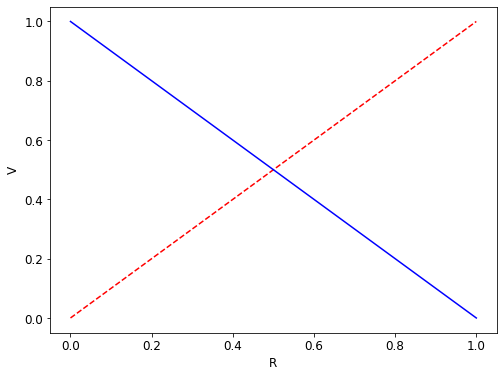
\includegraphics[scale=0.25]{img/slide/conint_illust.png}
        \label{fig:conint}
    \end{figure}
\end{frame}


\subsection{Research framework}
\begin{frame}{Research framework}
    \begin{figure}
        \centering
        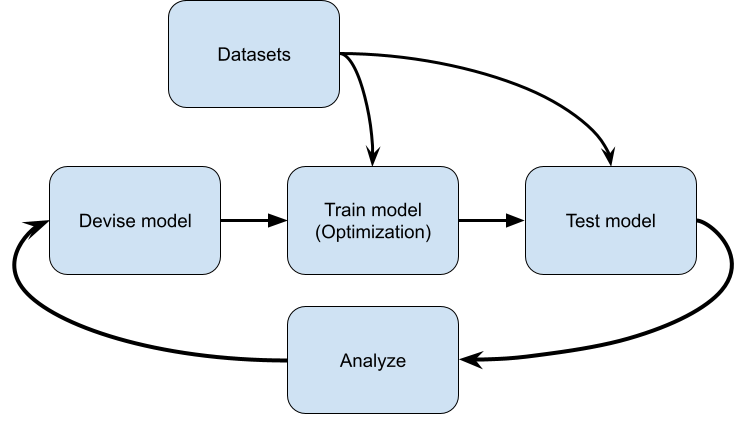
\includegraphics[scale=0.4]{img/slide/research_framework.png}
        \label{fig:framework_diagram}
    \end{figure}
\end{frame}


\section{Related work}
\begin{frame}{Section 2 overview}
    \tableofcontents[sections={2}]
\end{frame}
\subsection{Pair potentials}
\begin{frame}{Lennard-Jones potential}
    \begin{columns}
        \begin{column}{0.6\textwidth}
            The "building block" of pair potential. Devised by \textsc{Lennard \& Jones} (1924). The \textbf{Lennard-Jonnes potential (LJ-pot)}:
            \begin{equation}
                V = 4\epsilon\left[\left(\frac{\sigma}{R}\right)^{12} - \left(\frac{\sigma}{R}\right)^{6} \right].
                \label{eq:lj}
            \end{equation}
            \begin{itemize}
                \item $\epsilon$: depth of the "well".
                \item $\sigma$: collision diameter.
                \item $O(R^{-12})$ term: repulsive potential.
                \item $O(R^{-6})$ term: attractive potential.
            \end{itemize}
        \end{column}
        \begin{column}{0.5\textwidth}
            \begin{figure}
                \centering
                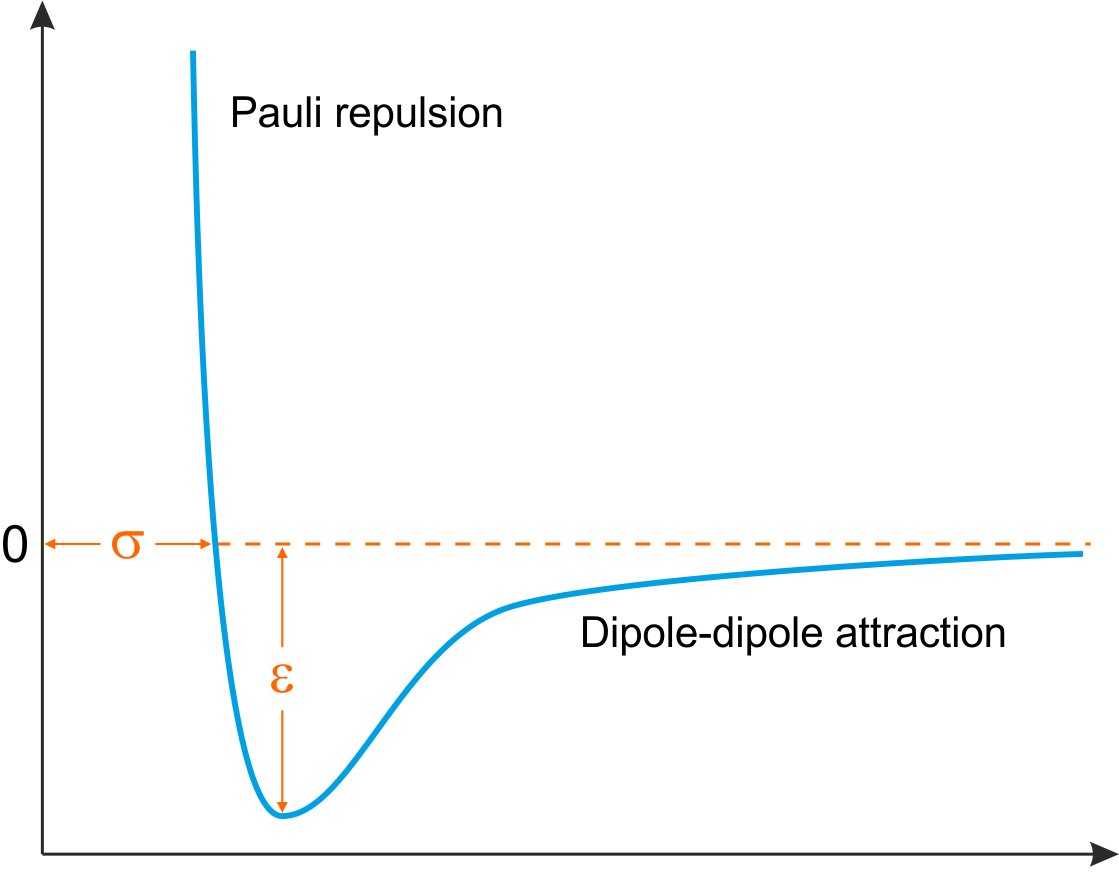
\includegraphics[scale=0.55]{img/slide/lennard_jones_potential.png}
                \label{fig:ljpot}
            \end{figure}
        \end{column}
    \end{columns}
\end{frame}
\begin{frame}{Morse \& Buckingham potential}
    \begin{itemize}
        \item Morse potential (1929): explicitly includes the effects of bond breaking
        \begin{equation}
            V = \epsilon(1-e^{-c_1(R-R_e)})^2.
        \end{equation}
        Drawback: too simple for modern spectroscopy.
        \item Buckingham potential (1938): improvement (more realistic) of the LJ-potential
        \begin{equation}
            V = c_1e^{-\alpha R} - \frac{c_2}{R^6}.
            \label{eq:buckingham}
        \end{equation}
        Drawback: infinitely attractive at $R \rightarrow 0$.
    \end{itemize}
\end{frame}
\begin{frame}{Modern pair potentials}
    \textsc{Pathak \& Thakkar} (1987) state that for monoatomic gases, the united-atom perturbation theory implies
    \begin{equation}
        V = c_1\frac{Z^2}{R} + c_2 + O(R^2) \quad \text{for }R \ll R_e.
        \label{eq:pathak}
    \end{equation}
    With exponential screening of the \textbf{Coulomb potential}, the functional form becomes
    \begin{equation}
        V = e^{-\alpha R}
        \left( c_1 \frac{Z^2}{R} 
        \left( 1 - \frac{(\alpha R)^2}{2} \right)
        + c_2(1+ \alpha R)\right) \quad \text{for }R \ll R_e,
        \label{eq:chargescreening}
    \end{equation}
\end{frame}
\begin{frame}{Modern pair potentials}
    A pair potential devised by \textsc{Deiters \& Neumaier} (2016) to correct the $R^{-6}$ behavior at large distances, the desired short-range behavior, and to avoid unrealistic (infinitely attractive) pole at $R \rightarrow 0$:
    \begin{equation}
        V = c_1 e^{-2\alpha R}\left(\alpha + \frac{1}{R}\right) - \frac{c_2R^2}{c_3 + R^8} + c_4,
        \label{eq:ljlike}
    \end{equation}
    where $\alpha$, $c_1$...$c_3 > 0$. \\
    
    A pair potential for noble gases, by \textsc{Deiters \& Sadus} (2019):
    \begin{equation}
        V = \frac{\left(\D\frac{c_0}{R}\right)e^{c_1R+c_6R^2} 
        + c_2e^{c_3R} + c_4}
        {1+ c_5R^6} + c_7.
    \end{equation}
\end{frame}

\subsection{PES from machine learning}
\begin{frame}{Neural network approach}
A global PES for H$_2$ + OH $\leftrightarrow$ H$_2$O + H reaction formed by \textbf{neural network (NN)} with two hidden layers is employed by \textsc{Chen} et al (2013). The general form:
    \begin{equation}
        y_{k,j} = f_k\left(b_{k,j} + \sum^{N_{k-1}}_{i=1}w_{k,j,i} y_{k-1,i}\right), \quad j=1,2,...,N_k,
        \label{eq:nnlayer}
    \end{equation}
    where $N_k$ indicates the number of neurons in the $k$th layer; $y_{k,j}$ is the output on the $k$th layer and $j$th node, if $k=0$, then $y_{0,i} = \mathbf{R}_i$.
\end{frame}

\subsection{Analytical PES}
\begin{frame}{Permutational-invariant PES}
By \textsc{Braams \& Bowman} (2009), for four atoms:
    \begin{equation}
        V = \sum^M_{\substack{a,b,c,d,e,f \\ a+b+c+d+e+f \leq M}}C_{abcdef}\left(y_{12}^a y_{13}^b y_{14}^c y_{23}^d y_{24}^e y_{34}^f\right),
        \label{eq:monomialc2h2}
    \end{equation}
    where
    \begin{equation}
        y_{ij} = \text{exp}(-r_{ij}/r_0)
        \label{eq:morse}
    \end{equation}
    is the Morse variable.
\end{frame}
\begin{frame}{CHIPR}
    \textbf{Combined hyperbolic inverse power representation (CHIPR)} by \textsc{Rocha \& Varandas} (2021) is state of the art global adiabatic PES, currently for up to tetratomics (A$_4$, AB$_3$, A$_2$B$_2$, ABC$_2$, ABCD molecules). The functional form is
    \begin{equation}
        V(\mathbf{r}) = \sum_i V_i^{(1)} + \sum_{i<j} V_{ij}^{(2)}(r_{ij}) + \sum_{i<j<k} V_{ijk}^{(3)}(r_{ij},r_{ik},r_{jk}) + ... ,
        \label{eq:chiprexpansion}
    \end{equation}
    also referred as the \textbf{many-body expansion}. The $n$-body term is
    \begin{equation}
        V^{(n)} = \sum^L_{i_1=0,...,i_\tau=0}C_{i_1,...,i_\tau}\prod^\tau_{p=1} y_p^{i_p},
        \label{eq:chiprnbody}
    \end{equation}
    where $y_p$ is a fixed function of coordinates.
\end{frame}
\begin{frame}{CHIPR for HO$_2^+$}
    By \textsc{Xavier} et al (2019), for global PES of HO$_2^+$. The functional form:
    \begin{equation}
        V = V^{(2)}_{\text{O$_2^+$}} + V^{(2)}_{\text{OH$^{+(1)}$}} + V^{(2)}_{\text{OH$^{+(2)}$}} +
        V^{(3)}_{\text{HO$_2^+$}}.
        \label{eq:ho2+chipr}
    \end{equation}
    The pair potential:
    \begin{equation}
        V^{(2)} = \frac{Z_iZ_j}{R}(C_1y_1 + C_2y_1^2 + C_3y_1^3).
        \label{eq:ho2+chiprv2}
    \end{equation}
    The 3-body potential:
    \begin{equation}
        \begin{split}
            V^{(3)} &= C_{110}y_1(y_2 + y_3) + 2C_{011}y_2y_3 +
            2C_{111}y_1y_2y_3 
            \\&+ C_{120}y_1(y_2^2 + y_3^2) + C_{210}y_1^2(y_2+y_3) + C_{012}(y_2y_3^2 + y_2^2y_3^2),
        \end{split}
        \label{eq:ho2+chiprv3}
    \end{equation}
    
\end{frame}
\begin{frame}{CHIPR for HO$_2^+$}
    \Fontvi
    \begin{equation}
        y_i =
        \begin{cases}
            \begin{cases}
                \D\sum_{k=1}^4 c_{1k}\text{ sech}^{\eta_{1k}}(\gamma_{1k}(\left[R_1 - \zeta_1(R_1^{\text{ref}})^{k-1}\right])) & \text{ for } V^{(2)}_{\text{OH}^+},\\
                \D\sum_{k=1}^4 c_{1k}(s_kR_1 + t_k)\text{ sech}^{\eta_{1k}}(\gamma_{1k}(\left[R_1 - \zeta_1(R_1^{\text{ref}})^{k-1}\right])) & \text{ for } V^{(2)}_{\text{O}_2^+}, \\
                \begin{split}
                    \D\sum_{k=1}^3 &c_{1k}(R_1^{\text{ref}})^{1-k}((\text{tanh}\left[\beta_1(R_1 - \zeta_1(R_1^\text{ref})^{k-1})\right]) \\ &\times \text{ sech}^{\eta_{1k}}(\gamma_{1k}\left[R_1 - \zeta_1(R_1^{\text{ref}})^{k-1}\right])), 
                \end{split}
                & \text{ for } V^{(3)}_{\text{HO}_2^+}, \\
            \end{cases}
            & \text{if }i=1, \\
                \begin{split}
                    \D\sum_{k=1}^3 &c_{ik}((\text{tanh}\left[\beta_i(R_i - \zeta_i(R_i^\text{ref})^{k-1})\right]) \\ & \times \text{sech}^{\eta_{ik}}(\gamma_{ik}\left[R_i - \zeta_i(R_i^{\text{ref}})^{k-1}\right])) \\ & \times {(R_i^{\text{ref}})^{1-k}}
                    & \text{ for all }V^{(2)} \text{ and } V^{(3)}, \\
                \end{split}
            & \text{ for } i=2,3.
            \end{cases}
        \label{eq:chipry}
    \end{equation}
\end{frame}
\begin{frame}{CHIPR for diabatic approximation}
    By \textsc{Xavier \& Varandas} (2021), to model the diabatic cusps of the double-sheeted PES of H$_2$O$^+$ dissociation. The functional form:
    \begin{equation}
        V_d = 
        \begin{bmatrix}
            V_{11} & V_{12} \\
            V_{21} & V_{22}
        \end{bmatrix}
        , V_{12} = V_{21}.
    \label{2x2diabaticmatrix}
    \end{equation}
    \begin{itemize}
        \item The diagonals are diabatic functions.
        \item The off-diagonals are coupling terms.
        \item Each term is modeled by adiabatic CHIPR.
    \end{itemize}
    The adiabatic potentials (eigenvalues):
    \begin{equation}
        V_{\pm} = \frac{V_{11} + V_{22}}{2} \pm \frac{1}{2}\sqrt{(V_{11} - V_{22})^2 + 4V_{12}^2},
        \label{2x2ev}
    \end{equation}
\end{frame}

\section{First results (fitting pair potentials)}
\begin{frame}{Section 3 overview}
    \tableofcontents[sections={3}]
\end{frame}
\subsection{Pair potential ansatz}
\begin{frame}{CHIPR pair potential}
    Generalized form of Eq.(\ref{eq:ho2+chiprv2}) and Eq.(\ref{eq:chipry}) with the total of $3(m + 1) + M$ adjustable parameters:
    \begin{equation}
        V = \frac{Z_iZ_j}{R^{\omega}}\sum_{k=1}^M C_ky_k,
        \label{eq:chiprv2general}
    \end{equation}
    \begin{equation}
        y_k = \D\sum_{p=1}^m c_{p}\text{ sech}^{\eta_{p}}(\gamma_{p}(\left[R - \zeta\beta^{p-1}\right])).
    \end{equation}
\end{frame}
\begin{frame}{Proposed pair potential}
    Rational ansatz with $3M+1$ adjustable parameters (\textbf{RATPOT1}). The functional form:
    \begin{equation}
        V = c_0 + P(R)/S(R),
        \label{eq:diatomicgeneralm}
    \end{equation}
    \begin{equation}
        P(R) = Z_iZ_j\left(\frac{1}{R}+ c_1 R\right)+c_2+c_3 R^2+ ...+c_{2M-1}R^{2M-2},
        \label{eq:diatomicgeneralm2}
    \end{equation}
    \begin{equation}
        Q(R)=1+(c_{2M}+c_{2M+1} R +...+c_{3M} R^M)R,
        \label{eq:diatomicgeneralm3}
    \end{equation}
    \begin{equation}
        S(R)=1+c_1 (R Q(R))^2,
        \label{eq:diatomicgeneralm4}
    \end{equation}
    where
    \begin{equation}
        c_1 > 0.
        \label{eq:diatomicgeneralm5}
    \end{equation}
\end{frame}
\begin{frame}{Proposed pair potential}
    (Experimental ver.) Rational ansatz with $4M+7$ adjustable parameters (\textbf{RATPOT2}). The functional form:
    \begin{equation}
        V_m(R)=c_0+P(R)/Q(R),
        \label{eq:ratpot2}
    \end{equation}
    \begin{equation}
        P(R)=c_1\prod_{i=1}^m ((R-a_i)^2+b_i R),
    \end{equation}
    \begin{equation}
        Q(R)=R(R+d_1)\prod_{i=2}^{m+3}((R-c_i)^2+d_i R),
    \end{equation}
    where $m>0$ and $b_i \ge 0 \text{ for } i>1$ and $d_i \ge 0 \text{ for } i>0$.
\end{frame}


\subsection{Data aspects}
\begin{frame}{Datasets}
    \begin{columns}
        \begin{column}{0.5\textwidth}
            Datasets for pair potential fitting:
            \begin{itemize}
                \item H$_2$ and its ions: 4 datasets.
                \item O$_2$ and its ions: 4 datasets.
                \item OH and its ions: 18 datasets.
            \end{itemize}
            
            Split dataset for training-testing or $k$-folds cross validation.
        \end{column}
        \begin{column}{0.5\textwidth}
            \begin{figure}[h]
                \centering
                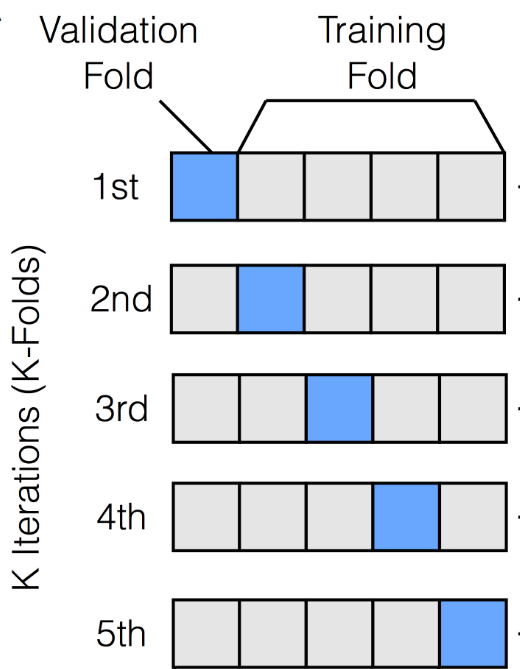
\includegraphics[scale=0.27]{img/slide/kfold.png}
                \label{fig:kfold}
            \end{figure}
        \end{column}
    \end{columns}
    
    
    
\end{frame}
\begin{frame}{Quality assessment}
    \begin{itemize}
        \item To assess the quality of the predictions, \textbf{root mean squared error (RMSE)} is used:
        \begin{equation}
            \text{RMSE} = \sqrt{\frac{1}{n}\sum_{i=1}^n \left[V(R_i) - V_{i,\text{ab initio}}\right]^2}.
            \label{eq:rmse}
        \end{equation}
        \item Computational efficiency assessment:
        \begin{equation}
            \overline{T_k} = \D\frac{\D\sum_{i=1}^m T_{k,i}}{m}.
            \label{eq:efficiency}
        \end{equation}
    \end{itemize}
\end{frame}


\subsection{Computational experiments}
\begin{frame}{Efficient formula evaluation}
    \Fontvi
    \begin{columns}[c]
        \begin{column}{0.5\textwidth}
            Algorithmic version of CHIPR (Eq.(\ref{eq:chiprv2general})):
            \begin{ppl}
            
                \vspace{0.2cm}
                Input: $C$, $R$, $Z$, $M$, $m$\\
                Output: $V$ \\
                $\omega := C_0$, $\zeta := C_1$, $\beta := C_2$ \\
                $\mu := [C_3...C_{m+2}]$ \\
                $\chi := [C_{m+3}...C_{2m+2}]$ \\
                $a := [C_{2m+3}...C_{3m+2}]$ \\
                $A := [C_{3m+3}...C_{3(m+1)+M}]$ \\
                $x := 0$, $R_{pow} := 1$\\ 
                for $i=0,1 ... m$, do:\\
                    \spc $\theta := (R - \zeta R_{pow})\mu_i$\\
                    \spc $x := x + (sech(\theta)^{\chi_i})a_i$\\
                    \spc $R_{pow} := R_{pow}\beta$\\
                end for \\
                $y := \text{horner}(x, A)x$\\
                $V := yZR^{-\omega}$
            \end{ppl}
        \end{column}
        \vrule{}
        \begin{column}{0.5\textwidth}
            Algorithmic version of RATPOT1  (Eq.(\ref{eq:diatomicgeneralm})):
            \vspace{0.2cm}
            \begin{ppl}
                
                Input: $C$, $R$, $Z$, $M$\\
                Output: $V$ \\
                if $C_1 < 0$: \\
                \spc $C_1 := -C_1$ \\
                end if \\
                $R_2 := R^2$ \\
                $K := [C_3 ... C_{2M-1}]$\\
                $y := \text{horner}(R, K)$\\
                $a := Z(1/R + C_1R) + C_2 + y$\\
                $K := [C_{2M} ... C_{3M}]$\\
                $y := \text{horner}(R, K)$\\
                $b := 1 + yR$\\
                $c := 1 + C_1(Rb)^2$\\
                $V := C_0 + a/c$, \\
            \end{ppl}
        \end{column}
    \end{columns}
\end{frame}
\iffalse
\begin{frame}{Efficient formula evaluation}
    \textbf{Horner's scheme}:
    Input: $x$, $C$ \\
    Output: $y$ \\
    $n := $ length of $C$ \\
    $y := C_n$ \\
    for $i=n-1, n-2 ... 0$, do: \\
    \spc $y := yx + C_i$ \\
    end for
\end{frame}
\fi
\begin{frame}{Optimization routine}
    \begin{columns}[c]
        \begin{column}{0.45\textwidth}
            \item The objective function:
            \begin{equation}
                F := \sum^n_{i=1}\left[V(R_i) - V_{i,\text{ab initio}}\right]^2.
                \label{eq:sumsquaredresidual}
            \end{equation}
        \end{column}
        \vrule{}
        \begin{column}{0.55\textwidth}
            \item The random multi-restart method, to find better solutions: \begin{enumerate}
                \item Generate random initial guess.
                \item Optimize using the guessed vector as initial point.
                \item Multiply the guessed vector with some factor.
                \item Repeat from 2.
            \end{enumerate}
        \end{column}
    \end{columns}
\end{frame}
\begin{frame}{Setups}
    \begin{itemize}
        \item Data: 4-fold cross validation for each dataset.
        \item Optimization method: local search methods (BFGS, Levenberg-Marquadt, etc). 
        \item Random multirestart: number of guesses = $10$, inner loop = $3$, factor $= 0.1$. 
        \item Time efficiency evaluation: $10^4$ evaluations, $m=20$.
        \item Programming language: Python 3.7.3.
        \item Hardware: AMD Ryzen 2600x 6/12 core/thread 4GHz.
    \end{itemize}
\end{frame}
\begin{frame}{Proposed ansatz vs CHIPR}
    \begin{figure}[h]
        %\centering
        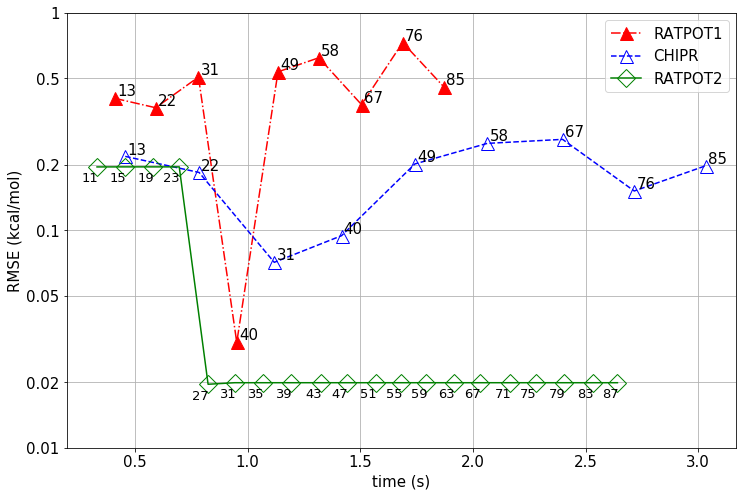
\includegraphics[scale=0.35]{img/slide/performance_ansatz0_vs_chipr_vs_ansatz2.png}
        \label{fig:perform}
    \end{figure}
\end{frame}
\begin{frame}{Proposed ansatz vs CHIPR}
    \begin{figure}[h]
        %\centering
        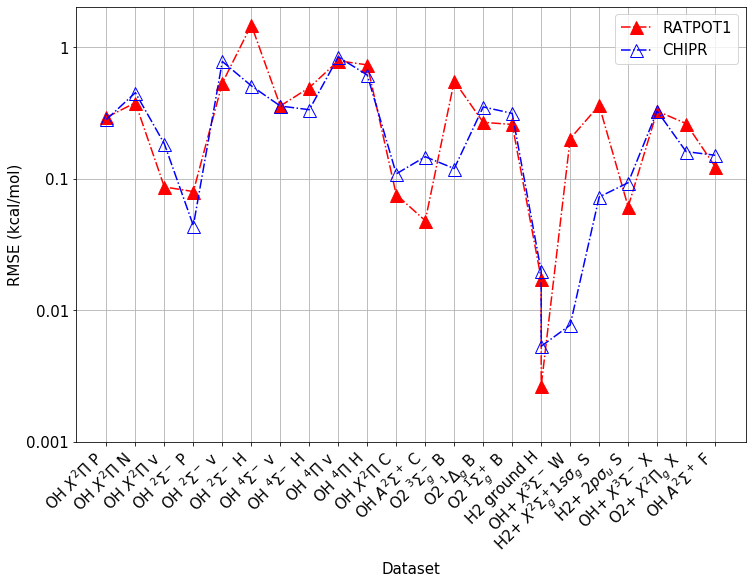
\includegraphics[scale=0.32]{img/slide/dataset_ansatz0_vs_chipr_v2.png}
        \label{fig:perform2}
    \end{figure}
\end{frame}


\section{Future work}
\begin{frame}{Section 4 overview}
    \tableofcontents[sections={4}]
\end{frame}


\subsection{PES for larger molecules}
\begin{frame}{Upscaling the PES}
    \begin{itemize}
        \item The target: $x + y \leq 60$.
        \item Challenges:
        \begin{itemize}
            \item Data aspects: 
            \begin{itemize}
                \item Requires thousands of \textit{ab initio} data points.
                \item Multi-sheeted PES datasets representing excited state energies. 
                \item Generate new \textit{ab initio} data points?
            \end{itemize}
            \item Model aspects:
            \begin{itemize}
                \item Representing permutation invariance property.
                \item Representing the long range interactions.
                \item Keeping the computational efficiency as low as possible despite larger molecular input features.
                \item Scales favorably with molecular system size.
                \item Multi-sheeted PES needs to represent multi-valued energies.
            \end{itemize}
        \end{itemize}
    \end{itemize}
\end{frame}

\begin{frame}{Upscaling the PES}
    Ideas:
    \begin{itemize}
        \item \textbf{Embedded atom model (EAM)} by \textsc{Daw \& Baskes} (1984):
        \begin{equation}
            V_i = F\alpha\left(\sum_{i<j}\rho_\beta(R_{ij})\right)+\frac{1}{2}\sum_{i<j}\phi_{\alpha\beta}(R_{ij}).
        \end{equation}
        \item NN-like functional form by \textsc{Behler} (2011):
        \begin{equation}
            V = \sum_i V_i(G_i(\mathbf{R})).
        \end{equation}
        \item Experiment with various extensions of the mentioned models.
    \end{itemize}
\end{frame}

\iffalse %%%%%%%%%%%%%%%%%%%%%%%%%%%
\begin{frame}{Upscaling the PES}
    \begin{itemize}
        \item The ideas:
        \begin{itemize}
            \item \textbf{Embedded atom model (EAM)} by \textsc{Daw \& Baskes} (1984):
            \begin{equation}
                V_i = F\alpha\left(\sum_{i<j}\rho_\beta(R_{ij})\right)+\frac{1}{2}\sum_{i<j}\phi_{\alpha\beta}(R_{ij}).
            \end{equation}
            \item 
        \end{itemize}
        \begin{itemize}
            \item $F$: represents energy required to place atom $i$ of type $\alpha$ into electron cloud.
            \item $\rho_\beta$: contribution of atom $j$ of type $\beta$ to electron charge density at the location of atom $i$.
            \item $\phi$: pair potential.
        \end{itemize}
    \end{itemize}
\end{frame}
\fi %%%%%%%%%%%%%%%%%%%%%%%%%%

\subsection{Optimization methods}
\begin{frame}{Optimization methods}
    \begin{columns}
        \begin{column}{0.6\textwidth}
        Ideas:
             \begin{itemize}
                \item Global optimization, e.g., SNOBFIT by \textsc{Huyer \& Neumaier} (2008).
                \item Ensemble of surrogate models , e.g., MADS-aggregate by \textsc{Audet et al} (2021).
            \end{itemize}
        \end{column}
        \begin{column}{0.5\textwidth}
            \begin{figure}[h]
                %\centering
                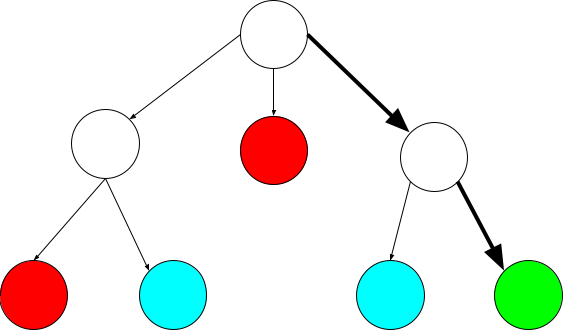
\includegraphics[scale=0.17]{img/slide/BnB.png}
                \label{fig:perform}
            \end{figure}
            \vspace{0.1cm}
            \begin{figure}[h]
                %\centering
                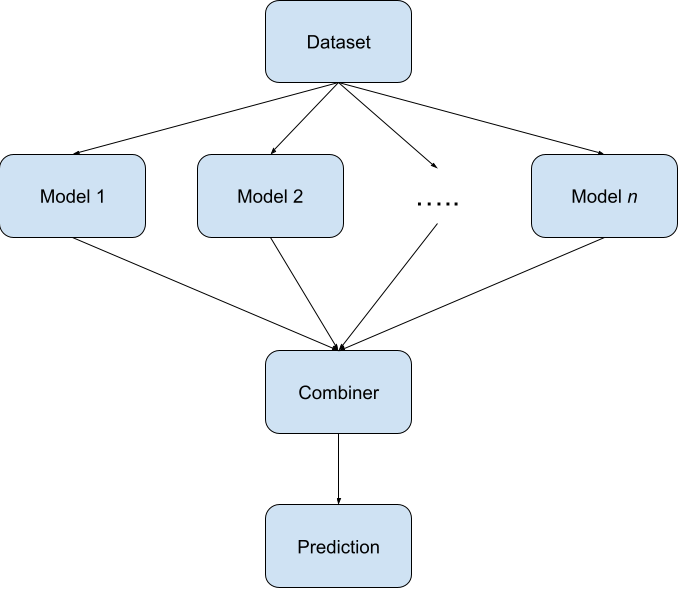
\includegraphics[scale=0.2]{img/slide/ensemble.png}
                \label{fig:perform}
            \end{figure}
        \end{column}
    \end{columns}
\end{frame}


\subsection{Multivalued fit}
\begin{frame}{Multivalued fit}
    The idea is to fit multi-valued datasets with a single formulation:
    \begin{equation}
        \min_\theta \sum F_i,
    \end{equation}
    where
    \begin{equation}
        F_i := \epsilon_i(\theta)^2,
    \end{equation}
    or
    \begin{equation}
        F_i := 1/\sum_k 1/\epsilon_{ik}(\theta).
    \end{equation}
    \begin{equation}
        \epsilon_i(\theta) = \min_k \left|\epsilon_{ik}(\theta)\right| = \min_k \left|y_i - \lambda_k(x_i, \theta)\right|.
    \end{equation}
\end{frame}

\iffalse
\subsection{Many-body-like potential}
\begin{frame}{Many-body-like potential}
Many-body-like potential which depends on other environmental variables.
    \begin{equation}
        \begin{split}
            V = \sum_i V_i + \sum_{i<j}\frac{Z_{ij}}{R}P - \sum_{i<j}\left(\frac{R}{Q}\right)^2, \\
            ...
        \end{split}
    \end{equation}
\end{frame}
\fi

\subsection{Finding conical intersections}
\begin{frame}{Conical intersection}
    \begin{itemize}
        \item Diabatic phenomena of PES.
        \item The intersection of two or more electronic states (in the shape of double cones).
        \item Only possible for molecules with more than 2 atoms (diatomic $\rightarrow$ \textbf{avoided crossing}).
        \item Guaranteed to occur from molecular symmetry, also has some possibilities to occur from non-symmetric molecules.
        \item Mathematically: when two or more eigenvalues of the PES matrix are degenerate.
        \item Applications: photophysics (photosynthesis), charge-transfer reactions, etc.
    \end{itemize}
\end{frame}
\begin{frame}{Conical intersection of two electronic states}
    \Fontvi
    The Hamiltonian:
    \begin{equation}
        \mathbf{H} = 
        \begin{pmatrix}
            H_{11} & H_{12} \\
            H_{21} & H_{22}
        \end{pmatrix},
        \label{eq:conintmat}
    \end{equation}
    where 
    \begin{equation}
        H_{ij} = \braket{\phi_i|H|\phi_j}.
    \end{equation}
    The eigenvalues:
    \begin{equation}
        E_{\pm} = \Bar{H} \pm \sqrt{\Delta H^2 + H_{12}^2},
    \end{equation}
    where
    \begin{equation}
        \Bar{H} = (H_{11} + H_{22})/2,
    \end{equation}
    \begin{equation}
        \Delta H = (H_{11} - H_{22})/2.
    \end{equation}
    The conditions for degeneracy:
    \begin{equation}
        H_{11} - H_{22} = 0,
    \end{equation}
    \begin{equation}
        H_{12} = 0,
    \end{equation}
\end{frame}


\begin{frame}{$N$-fold degeneracy rule}
    \Fontvi
    (From \textsc{Katriel \& Davidson} (1980)) For an $N \times N$ matrix, $N$-fold degeneracy requires to satisfy $N-1$ diagonal conditions
    \begin{equation}
        H_{11} = H_{22} = ... H_{NN},
    \end{equation}
    and $N(N-1)/2$ off diagonal conditions
    \begin{equation}
        H_{12} = H_{13} = ... H_{1N} = H_{N-1,N} = 0,
    \end{equation}
    which sums to $(N-1)(N+2)/2$ conditions. The maximum degeneracy of a molecule with $k^\text{int}$ degrees of freedom is given by the largest $N$ satisfying the inequality
    \begin{equation}
        (N-1)(N+2)/2 \leq 3k-6.
    \end{equation}
\end{frame}
\iffalse %%%%%%%%%%%%%%%
\begin{frame}{Conical intersection example}
    A symmetric $3 \times 3$ matrix:
    \begin{equation}
        A(s,t)=
        \begin{pmatrix}
            t & 2t+s & t+1 \cr 2t+s & 2t & t+1 \cr t+1 & t+1 & t+1-s
        \end{pmatrix}
        .
    \end{equation}
    The conical intersection is found at $(s,t)=(2,-1)$ where the matrix becomes diagonal with a double eigenvalue.
\end{frame}
\begin{frame}{Conical intersection example}
    \begin{figure}[h]
        \centering
        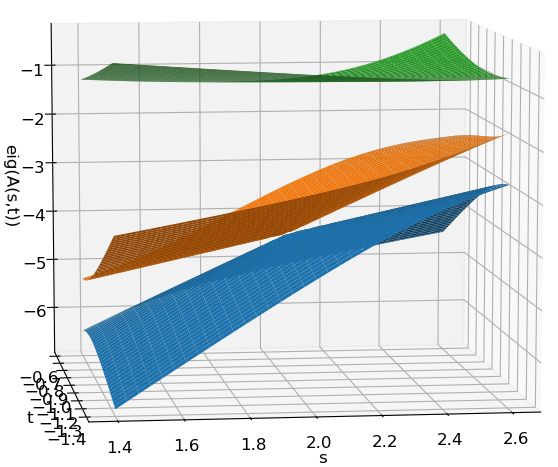
\includegraphics[scale=0.5]{img/slide/conint_3sheet_angle9.png}
        \label{fig:conint}
    \end{figure}
\end{frame}
\begin{frame}{Conical intersection example}
    \begin{figure}[h]
        \centering
        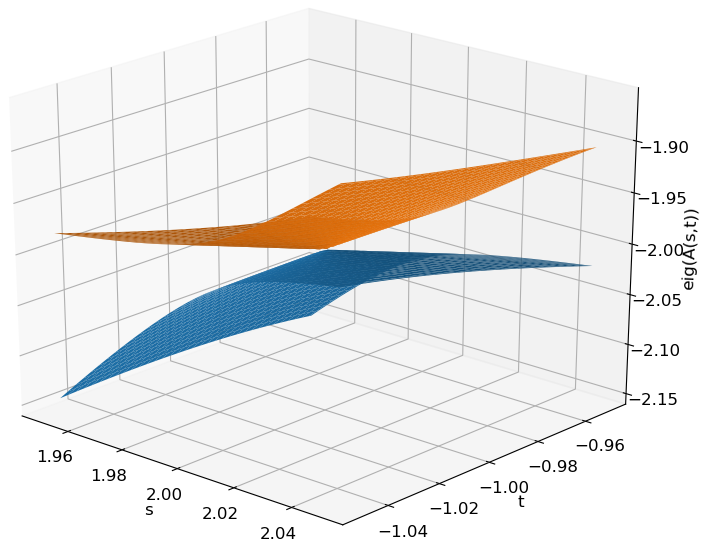
\includegraphics[scale=0.5]{img/slide/conint_3sheet_angle8.png}
        \label{fig:conint}
    \end{figure}
\end{frame}
\fi %%%%%%%%%%%%%%%%%
\begin{frame}{Conical intersection example}
    A symmetric $3 \times 3$ matrix:
    \begin{equation}
        A(s,t)=
        \begin{pmatrix}
            3-s & s+t & -s-t \cr s+t & s-t & s^2-1 \cr -s-t & s^2-1 & 3-s
        \end{pmatrix}
        .
    \end{equation}
    The conical intersections are found at $(s,t)=(1,-1)$ and $(s,t) = (-1, 1)$.
\end{frame}
\begin{frame}{Conical intersection example}
    \begin{figure}[h]
        \centering
        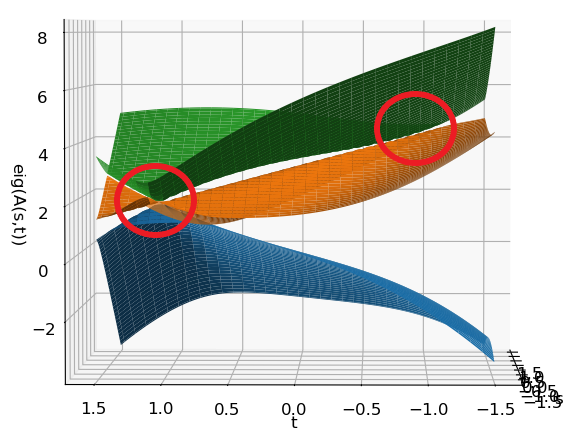
\includegraphics[scale=0.5]{img/slide/conint_3sheet_angle10.png}
        \label{fig:conint}
    \end{figure}
    \nocite{*} %for bib
\end{frame}

\begin{frame}[shrink=50]{References}
    \tiny
    \printbibliography
\end{frame}



\end{document}